\documentclass[12pt, a4paper]{article}
\usepackage{graphicx}
\usepackage{listings}
\usepackage{xcolor}
\graphicspath{{images/}}
\usepackage[utf8]{inputenc}
\usepackage[english]{babel}
\usepackage{alphabeta}
\usepackage{tcolorbox}
\usepackage[total={6.5in, 9.2in}]{geometry}
\usepackage{subfig}
\usepackage{amsmath}
\usepackage{hyperref}
\usepackage{lastpage}
\usepackage{fancyhdr}
\captionsetup[figure]{name=Εικόνα}
\usepackage{fancyhdr}
\usepackage{pgfplots}
\usepackage{tikz}

\hypersetup{
	colorlinks,
	citecolor=black,
	filecolor=black,
	linkcolor=black,
	urlcolor=black
}
\definecolor{cosmiclatte}{rgb}{1.0, 0.97, 0.91}
\lstdefinestyle{text}{
	basicstyle=\ttfamily\footnotesize,
	numbers=left,
	numberstyle=\tiny\color{gray},
	stepnumber=1,
	numbersep=5pt,
	backgroundcolor=\color{cosmiclatte},
	showspaces=false,
	showstringspaces=false,
	showtabs=false,
	tabsize=2,
	captionpos=b,
	breaklines=true,
	breakatwhitespace=true,
	breakautoindent=true,
	breakindent=30pt,
	keywordstyle=\color{blue},
	commentstyle=\color{green!40!black},
	stringstyle=\color{red},
	morecomment=[l][\color{magenta}]{\#}
}


\begin{document}
	
	
	\thispagestyle{empty}
	
	\begin{center}
		
		
		\begin{tabular}{c}
			\hline \\
			\Huge \textbf{Κατανεμημένα Συστήματα}\\[0.5em]
			\hline
		\end{tabular}\\[5em]
		
		
		
		\LARGE \textbf{Εξαμηνιαία Εργασία} \\[0.5em]
		\Large BlockChat \\[1em]
	
		
		\small [Το \foreignlanguage{english}{\LaTeX} Project
		\href{https://www.dropbox.com/scl/fi/jr7wfars2906nf6gk16gz/reportDistributedSystems.zip?rlkey=78r426g8wb01vbl8f1m0rhvgi&dl=0}{\color{purple} \textbf{εδώ}}] \\[7em]
		
		\Large \textbf{Ομάδα 29}\\[0.3em]
		\large Δημήτριος-Δαυίδ Γεροκωνσταντής (ΑΜ : 03119209)\\
		\large Αθανάσιος Τσουκλείδης-Καρυδάκης (ΑΜ : 03119009)\\
		\large Ιωάννης Καραυγουστής (ΑΜ : 03119847)\\[7em]
		\large
		\textbf{Εαρινό 2024}\\[3.1em]
		
		\includegraphics[width=1.5in]{NTUA}\\[1em]
		\large
		
		Εθνικό Μετσόβιο Πολυτεχνείο\\
		Σχολή ΗΜΜΥ
	\end{center}
	
	\begingroup
	\let\cleardoublepage\clearpage
	\tableofcontents
	\endgroup
	\newpage
	
	\section*{Εισαγωγή}
	Σκοπός αυτής της εργασίας είναι η σχεδίαση και υλοποίηση μιας εφαρμογής βασισμένης στην τεχνολογία του Blockchain. Συγκεκριμένα πρόκειται για ένα κατανεμημένο σύστημα μέσω του οποίου διάφοροι χρήστες μπορούν να επιτελέσουν δύο λειτουργίες σε μορφή transactions : 
	\begin{enumerate}
		\item Ανταλλαγή μηνυμάτων 
		\item Μεταφορά χρημάτων
	\end{enumerate}
	Σκοπός είναι να επιτευχθεί η ορθή και συνεπής λειτουργία του συστήματος κάτω από πραγματικές συνθήκες χρήσης από πολλαπλούς participants ταυτόχρονα, όπου το σύστημα επιβαρύνεται με πολλά παράλληλα transactions. Προφανώς, σκοπός είναι και η υλοποίηση των βασικών δομικών χαρακτηριστικών της τεχνολογίας του blockchain που αφορούν την αυτόνομη αλλά και συνεπή λειτουργία των κόμβων με όλους τους απαραίτητους μηχανισμούς επικύρωσης των transactions και των blocks που δημιουργούνται.
	Η παρούσα αναφορά χωρίζεται στα παρακάτω τρία κεφάλαια :
	\begin{enumerate}
		\item \textbf{Κεφάλαιο 1\textsuperscript{ο}}: Παρουσίαση της δομής του κατανεμημένου συστήματος και των βασικών λειτουργιών του BlockChat. Αναφορά σε επιπλέον χαρακτηριστικά που υλοποιήθηκαν με σκοπό την ορθότερη λειτουργία του κατανεμημένου συστήματος.
		\item \textbf{Κεφάλαιο 2\textsuperscript{ο}}: Παρουσίαση του Frontend και του CLI. 
		\item \textbf{Κεφάλαιο 3\textsuperscript{ο}}: Παρουσίαση των αποτελεσμάτων των μετρήσεων που πραγματοποιήθηκαν με χρήση VMs από την cloud υπηρεσία του okeanos-knossos.
	\end{enumerate}
	\section{Δομή και λειτουργικότητα του BlockChat}
	Στο κεφάλαιο αυτό παρουσιάζεται αρχικά η αρχιτεκτονική δομή του συστήματός μας, τα εργαλεία που χρησιμοποιήθηκαν για την υλοποίησή του καθώς και οι λειτουργικότητές του. Να σημειωθεί ότι για την υλοποίηση του BlockChat backend χρησιμοποιήθηκε η python flask.
	\subsection{Δομή-Αρχιτεκτονική του BlockChat}
	Η δομή του κατανεμημένου συστήματος που υλοποιούμε φαίνεται στην εικόνα \ref{fig:components}, όπου παρουσιάζονται τα βασικά δομικά χαρακτηριστικά των κόμβων του BlockChat καθώς και του τρόπου επικοινωνίας μεταξύ τους. Όπως φαίνεται στο σχήμα για 3 κόμβους συνολικά, κάθε participant του blockchat περιέχει:
	\begin{enumerate}
		\item ένα component που διαχειρίζεται τα εισερχόμενα transactions (Transactions Receiver)
		\item ένα component (Transactions Creator) που δημιουργεί και προωθεί νέα transactions σε ένα component (Broadcaster) που υλοποιεί την broadcast αποστολή τους στους άλλους συμμετέχοντες
		\item Έναν μηχανισμό proxy ο οποίος διαχειρίζεται εισερχόμενα requests, δηλαδή εισερχόμενα transactions.
	\end{enumerate}
		\begin{figure}[h!]
		\centering
		\includegraphics[width=6.5in]{components.png}
		\caption{Δομικά χαρακτηριστικά του BlockChat}
		\label{fig:components}
	\end{figure}
	Ο τρόπος λειτουργίας των πρώτων δύο components που υλοποιούν ουσιαστικά την λογική του BlockChat θα παρουσιαστεί στην συνέχεια. Ως προς τη δομή του συστήματος, ενδιαφέρον έχει η παρουσίαση της λειτουργικότητας του proxy. Η ουσία έγκειται στον πλήρη διαχωρισμό (decoupling) της υλοποίησης της λογικής του BlockChat από την επικοινωνία μεταξύ των κόμβων. Έτσι, κάθε κόμβος blockchat επιφορτίζεται μόνο με την διαχείριση των transactions και του blockchain, ενώ ο proxy είναι αυτός που αναλαμβάνει να δέχεται εισερχόμενα transactions από τους υπόλοιπους κόμβους και να τα προωθεί στα αντίστοιχα components του κόμβου με συγκεκριμένο ρυθμό και σειριακά. Πρακτικά, αυτό που συμβαίνει είναι ότι όταν ένας κόμβος δημιουργεί ένα transaction και το προωθεί σε όλους τους άλλους κόμβους, στην πραγματικότητα αυτό το transaction λαμβάνεται από τον proxy κάθε μηχανήματος (όπως και από τον δικο μας proxy). Έτσι τόσο για τα transactions που δημιουργεί ένας κόμβος όσο και για αυτά που λαμβάνει από τους υπόλοιπους κόμβους, υπάρχει ο proxy ώστε όλα αυτά τα transactions να τα αποθηκεύει σε μια ουρά και να τα προωθεί αυτός στο εσωτερικό του κόμβου προκαλώντας την λειτουργία της λογικής του blockchat. Όπως γίνεται αντιληπτό, για την διαχείριση των σύγχρονων transactions (υπενθυμίζεται ότι στο συστημά μας, δημιουργούνται παράλληλα transactions από όλους τους κόμβους και κάθε κόμβος οφείλει να ενημερώνει την κατάστασή του τόσο βάσει των δικών του transactions όσο και βάσει των transactions των υπολοίπων), ακολουθήσαμε τη λογική της σειριοποίησής τους. Όλα τα transactions που συσσωρεύονται στην ουρά του proxy, προωθούνται σειριακά στο σύστημα και εκτελούνται ατομικά. Κάθε επόμενο transaction προωθείται στο σύστημά μας αφότου έχει πλήρως εξυπηρετηθεί το προηγούμενο transaction. Με αυτό τον τρόπο το state κάθε κόμβου παραμένει συνεπές και ορθό. Ωστόσο, αυτή η λογική σειριοποίησης απαιτούσε και κάποιες επιπλέον προσθήκες στην υλοποίηση του BlockChat για λόγους συγχρονισμού και επιβολής συγκεκριμένης σειράς με την οποία εκτελούνται οι επιμέρους λειτουργίες. Για παράδειγμα όταν ένα block γίνεται mine και ο validator πρέπει να κάνει broadcast το block του, χρειάστηκε να εξασφαλιστεί ότι έχει ολοκληρωθεί το broadcast προτού ο validator αρχίζει να δέχεται νέα transactions, διαφορετικά θα υπήρχε ασυνέπεια σε μεταβλητές κατάστασης που διατηρεί ο εν λόγω κόμβος. Ένα δεύτερο παράδειγμα τέτοιου χειρισμού είναι ότι έπρεπε να διασφαλιστεί ότι πρώτα θα ενημερωθεί το state ενός κόμβου με βάση το τελευταίο transaction ενός block και μετά θα γίνει η αναίρεση του state και ο επανυπολογισμός του βάσει του block που στέλνει ο validator. Διαφορετικά, επίσης θα υπήρχε έλλειψη ορθότητας (η οποία παρατηρήθηκε χωρίς αυτή την παρέμβαση).Τέλος, σημειώνουμε ότι η επικοινωνία μεταξύ των κόμβων γίνεται μέσω REST API που δημουργήθηκε με χρήση της βιβλιοθήκης flask της python.
		\begin{figure}[t!]
		\centering
		\includegraphics[width=6.5in]{bootstraping.png}
		\caption{Σχηματική αναπαράσταση του Bootstraping για blockchat με 5 κόμβους}
		\label{fig:bootstraping}
	\end{figure}
	\subsection{Λειτουργικότητα}
	Στο BlockChat θεωρούμε ότι υπάρχει ένας κόμβος, ο bootstraping node, ο οποίος ενώ είναι ισότιμος κόμβος με τους υπόλοιπους, κατά την αρχικοποίηση του συστήματος αναλαμβάνει τις εξής βασικές λειτουργίες:
	\begin{enumerate}
		\item Πρόκειται για έναν κόμβο με γνωστή IP σε όλους τους υπόλοιπους. Ο bootstraping node οφείλει να δέχεται αιτήματα για register από τους υπόλοιπους participants ώστε να τους εισάγει επιτυχώς στο blockchat κατά τη διαδικασία αρχικοποίησης. Σε κάθε νέο κόμβο που επικοινωνεί με αυτόν, αναλαμβάνει να τον ενημερώσει για το public key του, να του δώσει το ήδη υπάρχον Blockchain, να του αναθέσει ένα id και να του μεταφέρει το αρχικό χρηματικό ποσό των 1000 coins.   
		\item Όταν και ο τελευταίος κόμβος εισάγεται στο σύστημα, ο bootstraping node αφού του μεταφέρει όσα και πριν, φροντίζει να ενημερώσει όλους τους participants με πληροφορίες για όλους τους υπόλοιπους participants ώστε μετά από αυτό το σημείο όλοι να γνωρίζουν όλους τους υπόλοιπους και να μπορούν να επικοινωνούν μεταξύ τους. 
	\end{enumerate}
	Αυτή η διαδικασία του bootstraping φαίνεται σχηματικά στην εικόνα \ref{fig:bootstraping} όπου έχει σχεδιαστεί ένα sequence διάγραμμα.

\noindent
	Για λόγους αφενός διευκόλυνσης και αφετέρου συνέπειας με τους περιορισμούς της εκφώνησης, αποφασίστηκε να μην επιτρέπεται στους κόμβους να στέλνουν μεταξύ τους transactions προτού εισαχθούν όλοι οι κόμβοι στο BlockChat. Δεδομένου ότι όλοι οι κόμβοι γνωρίζουν τους υπόλοιπους μόνο στο τέλος του bootstraping, η broadcast αποστολή transactions σε κόμβους που ακόμη δεν είναι γνωστοί δημιουργεί πρόβλημα στην ενημέρωση του state καθώς οι κόμβοι που λαμβάνουν τέτοια transactions δεν γνωρίζουν ενδεχομένως τους εμπλεκόμενους σε αυτά. Επιπλέον, ακόμη κι αν υλοποιούσαμε κάτι τέτοιο, transactions αυτού του τύπου θα μπορούσαν να στέλνονται μόνο στον bootstraping κόμβο, καθώς πριν την εισαγωγή όλων των κόμβων, κάθε κόμβος γνωρίζει μόνο τον bootstraping και μόνο με αυτόν θα μπορούσε ενδεχομένως να ανταλλάξει transactions. Τέλος, ως προς το bootstraping αξίζει να σημειωθεί ότι ο bootstraping node είναι έτσι υλοποιημένος ώστε η διαδικασία της αποστολής των 1000 coins, του chain και των συνολικών πληροφοριών στο τέλος να γίνεται από ένα άλλο νήμα (χρήση της βιβλιοθήκης threading στην python). 
		\begin{figure}[b!]
		\centering
		\includegraphics[width=7in]{activityDiagram.png}
		\caption{Λειτουργικότητα ενός BlockChat κόμβου}
		\label{fig:activity}
	\end{figure}
	\noindent
	Στη συνέχεια, παρουσιάζεται η βασική λειτουργικότητα κάθε κόμβου του blockchat. Αυτή η λειτουργικότητα παρουσιάζεται αρκετά αναλυτικά στο activity diagram της εικόνας \ref{fig:activity}. Συγκεκριμένα κάθε κόμβος ταυτόχρονα δημιουργεί νέα transactions και δέχεται άλλα transactions που δημιουργούνται από άλλους κόμβους. Η διαδικασία από έκει και έπειτα περιγράφεται περιεκτικά στο διάγραμμα αλλά αξίζει να σημειωθούν τα εξής :
	\begin{itemize}
		\item Όταν ένας κόμβος δέχεται ένα block από τον validator, το επικυρώνει. Αυτη η διαδικασία ενώ θα μπορούσε να γίνει αρκετά πλήρης και περίπλοκη, ακολουθήσαμε την υπόδειξη της εκφώνησης σύμφωνα με την οποία το validation αφορά την επαλήθευση του previous hash καθώς και του αποστολέα (αν πράγματι είναι ο εκλεγμένος από όλους validator). Δηλαδή δεν γίνεται κάποιο parse του block για επαλήθευση των transactions που περιλαμβάνει.
		\item Κάθε κόμβος διατηρεί ένα state για την κατάσταση του blockchat (π.χ. τα balances όλων των κόμβων, τα επόμενα nonces που περιμένει να λάβει από κάθε κόμβο, τα stakes τους κλπ). Όταν ένα block γίνεται mine, ο validator απλώς διατηρεί το state του καθώς τελικά αυτό θα επικρατήσει σε όλους. Ωστόσο, μέχρι να γίνει mine αυτό το block, στο μεταξύ οι υπόλοιποι κόμβοι που χτίζουν το δικό τους block ενδέχεται να έχουν διαφορετική εντύπωση για το state του συστήματος. Ως μη validators, όλοι αυτοί οι κόμβοι οφείλουν να υιοθετήσουν την άποψη του validator. Συγκεκριμένα, από κάθε κόμβο διατηρούνται κάποια checkpoints (ουσιαστικά κατά την μετάβαση σε νέο block) με το state του, έτσι ώστε αν δεν είναι vaidator, να επιστρέψει στο προηγούμενο state του (δηλαδή να κάνει rollback τις αλλαγές που έχει προκαλέσει σε αυτό) και να κάνει rerun όλα τα transactions που περιέχονται στο received validated block.
	\end{itemize}
	\subsection{Διαχείριση Stake}
	Ως προς τη λειτουργικότητα του συστήματος, αξίζει να αναφερθεί ο τρόπος διαχείρισης του stake των κόμβων. Δεδομένου ότι η οποιαδήποτε αλλαγή σε stake αποτελεί ένα transaction, θεωρήθηκε χρήσιμο και δίκαιο η αλλαγή αυτή να γίνει εμφανής στους κόμβους μόνο μετά το mining του block που περιλαμβάνει το εν λόγω transaction. Συνεπώς, αν σε ένα block εισαχθεί ένα transaction αλλαγής stake, η χρήση του νέου stake θα χρησιμοποιηθεί για το mining του επόμενου και όχι του παρόντος block. Ωστόσο, ακόμα και με αυτή την υλοποίηση υπάρχει ακόμη πρόβλημα. Αν στο μέσο ενός block κάποιος κόμβος με balance 500 αποφασίζει να εισαγάγει ένα transaction αλλαγής stake σε 400, οι υπόλοιποι κόμβοι που λάβουν με broadcast τρόπο αυτό το transaction προφανώς θα το επικυρώσουν. Ωστόσο, έστω ότι αυτός ο κόμβος προτού γεμίσει το συγκεκριμένο block εισάγει ένα νέο transaction μεταφορά 200 coins σε κάποιον άλλο. Δεδομένου ότι το stake 400 ακόμη δεν έχει ενημερώσει την κατάσταση των κόμβων, αυτό το transaction θα επικυρωθεί επίσης. Έτσι, ο εν λόγω κόμβος κατάφερε και να αυξήσει το stake του (αυξάνοντας την πιθανότητα να γίνει αργότερα validator) και κατάφερε να κάνει transactions που υπερβαίνουν αυτό το stake. Για την επίλυση αυτού του φαίνομένου, οι κόμβοι (είτε όταν λαμβάνουν είτε όταν κάνουν broadcast ένα νέο block) εντοπίζουν τα stake transactions που περιλαμβάνονται σε αυτό και αφότου ενημερώσουν στο state τους με όλα τα υπόλοια transactions του block, στο τέλος ελέγχουν ξανά ότι το συγκεκριμένο transaction αλλαγής stake εξακολουθεί να είναι έγκυρο. Αν είναι έγκυρο, τότε πράγματι ενημερώνουν το stake του κόμβου, διαφορετικά δεν επικυρώνουν αυτή την αλλαγή.  

	\section{CLI και Frontend}
	Στο κεφάλαιο αυτό, παρουσιάζεται το CLI και το Frontend που δημιουργήθηκαν στα πλαίσια της παρούσας εργασίας. 
	\subsection{CLI}
	Μέσω του CLI, κάθε blockchat κόμβος έχει τη δυνατότητα να στέλνει transactions για messages ή coins, να βλέπει το balance του, να βλέπει το τελευταίο validated block του blockchain και τον validator του και να μεταβάλλει το stake του. Συγκεκριμένα, με χρήση της εντολής bchelp, βλέπουμε το description και τη χρήση κάθε τέτοιας εντολής:
	\begin{lstlisting}[style=text]
This is a description of how to use this CLI

1st command
t <recipient address> <message>
Description: It sends the message <message> to the node with id=<recipient_address>

2nd command
c <recipient address> <amount>
Description: It sends <amount> coins to the node with id=<recipient_address>

3rd command
stake <amount>
Description: It updates the stake so as to be equal to <amount> coins

4th command
view
Description: It prints the last validated block of the blockchain and the validator of it

5th command
balance
Description: It prints the balance of the node
	\end{lstlisting}
Το CLI δημιουργήθηκε με χρήση της βιβλιοθήκης click της python. Για κάθε αρχείο .py που δημιουργήθηκε για κάθε μια από τις εντολές του CLI, χρειάστηκε η εκτέλεση των παρακάτω:
\begin{lstlisting}[style=text]
sudo nano /usr/local/bin/<command_name>
	
	Inside this file, write:
	python3 <path_to_cli_py_file> "$@"

chmod +x /usr/local/bin/<command_name>
\end{lstlisting}
Επίσης με 
\begin{lstlisting}[style=text]
<command_name> --help
\end{lstlisting}
μπορεί κανείς να διαβάσει πληροφορίες χρήσης της εκάστοτε εντολής.
\subsection{Frontend}
\begin{figure}[h!]
	\centering
	\includegraphics[width=7in]{sc1.png}
	\caption{Αρχική σελίδα Frontend}
	\label{fig:landingPage}
\end{figure}
\noindent
Στη συνέχεια, παρουσιάζεται το frontend (χρήση React.js) μέσω του οποίου κάθε κόμβος μπορεί να πραγματοποιήσει όλες τις βασικές λειτουργίες του BlockChat. Η αρχική σελίδα φαίνεται στην εικόνα \ref{fig:landingPage}. Μέσω αυτής της σελίδας, ο χρήστης μπορεί να δημιουργήσει νέα message και coins transactions εισάγοντας το περιεχόμενο του transaction (coins ή message) και το id του receiver (για λόγους απλότητας, όχι το public key του). Επιπλέον μπορεί να δει το balance του. 
\begin{figure}[h!]
	\centering
	\includegraphics[width=7in, height=3.5in]{sc4.png}
	\caption{Outgoing Messages Page}
	\label{fig:showMessages}
\end{figure}
\begin{figure}[h!]
	\centering
	\includegraphics[width=7in,height=3.5in]{sc7.png}
	\caption{Money Transfers Page}
	\label{fig:showMoneyTrans}
\end{figure}
Επιλέγοντας Show Messages, προωθείται στην σελίδα που φαίνεται στην εικόνα \ref{fig:showMessages}. Εδώ, μπορεί να δει τα μηνύματα που έχει στείλει (outgoing messages) και με χρήση του κατάλληλου button να δει τα μηνύματα που έχει παραλάβει (ingoing messages). Ομοίως, με την επιλογή Show Money Transfers, οδηγούμαστε στη σελίδα που φαίνεται στην εικόνα \ref{fig:showMoneyTrans} όπου κανείς μπορεί να δει εισερχόμενα και εξερχόμενα coin transactions.
Τέλος, με χρήση της επιλογής Mining, οδηγούμαστε στην σελίδα της εικόνας \ref{fig:miningPage} από όπου μπορούμε να δούμε και να αλλάξουμε το stake, να δούμε πόσα blocks έχουμε κάνει εμείς mine, πόσα transactions απομένουν για να γεμίσει το επόμενο block και έναν κατάλογο που περιλαμβάνει για τα blocks που έχουμε κάνει mine, την θέση τους στο blockchain και το συνολικό fee που εισπράξαμε από το mining αυτών.
\begin{figure}[h!]
	\centering
	\includegraphics[width=7in]{sc6.png}
	\caption{Mining Page}
	\label{fig:miningPage}
\end{figure}
\\Για την χρήση του frontend θα χρειαστεί η εκτέλεση των εντολών npm install και npm start εντός του φακέλου όπου βρίσκεται το frontend.
	\section{Μετρήσεις και αποτελέσματα}
	\begin{figure}[b!]
		\centering
		\subfloat[With Sleep]{
			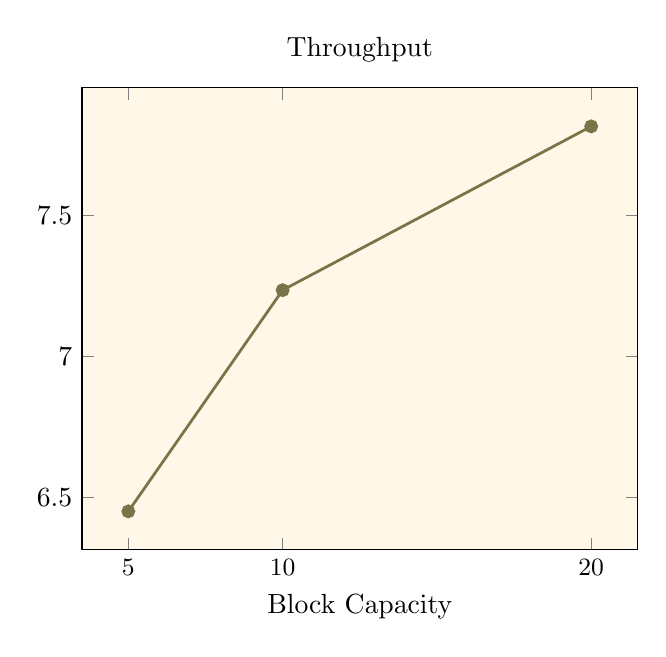
\begin{tikzpicture}
				\begin{axis}[xlabel={Block Capacity},
					title={Throughput},xtick={5,10,20}, xticklabel style={font=\small} ,width=3.4in,axis background/.style={fill=cosmiclatte}]
					\addplot[mark=*,yellow!40!black, line width=1pt]coordinates{
						(5,500/77.52293920516968)
						(10,500/69.10346174240112)
						(20,500/63.95952773094177)
					};
				\end{axis}
			\end{tikzpicture}
			
		}
		\subfloat[Without Sleep]{
			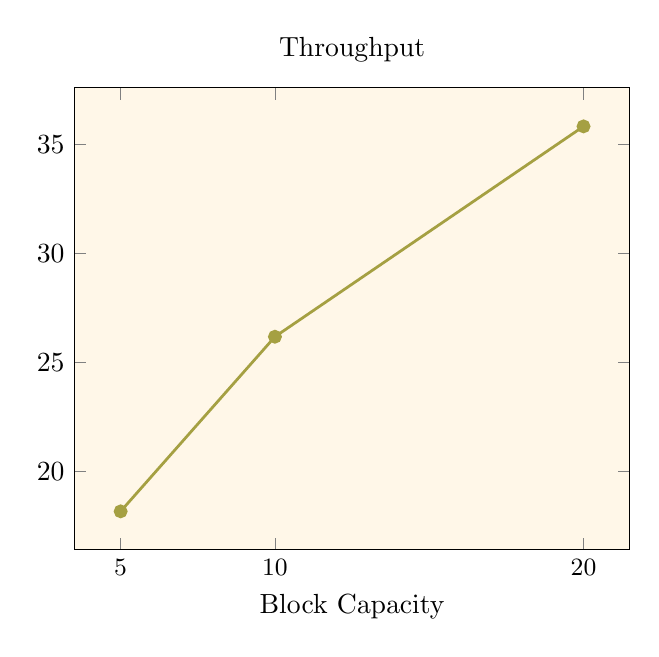
\begin{tikzpicture}
				\begin{axis}[xlabel={Block Capacity},
					title={Throughput},xtick={5,10,20}, xticklabel style={font=\small} ,width=3.4in,axis background/.style={fill=cosmiclatte}]
					\addplot[mark=*,yellow!60!black, line width=1pt]coordinates{
						(5,500/27.52293920516968)
						(10,500/19.10346174240112)
						(20,500/13.95952773094177)
					};
				\end{axis}
			\end{tikzpicture}
			
		}
		
		\caption{Throughput με block capacities = $\{5, 10, 20\}$, 5 clients και stakes ίσα με 10 για όλους.}
		\label{fig:diagram1}
	\end{figure}
	
	
	\begin{figure}[b!]
		\centering
		\subfloat[With Sleep]{
			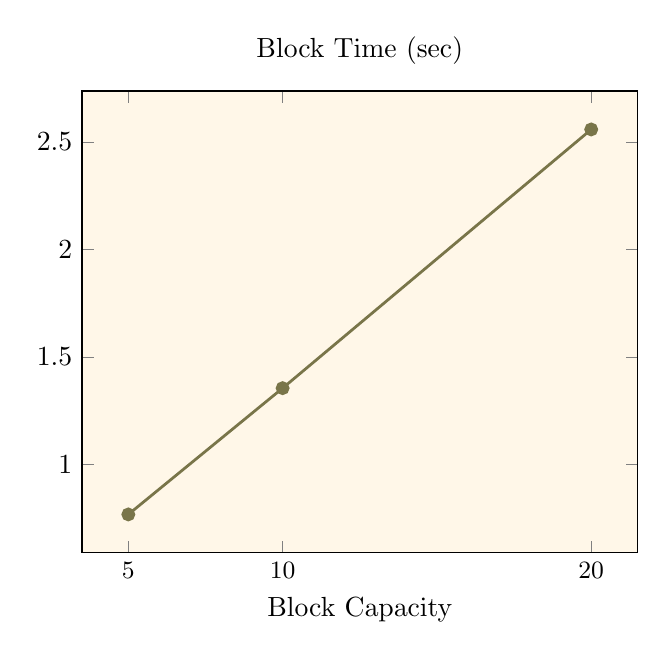
\begin{tikzpicture}
				\begin{axis}[xlabel={Block Capacity},
					title={Block Time (sec)},xtick={5,10,20}, xticklabel style={font=\small} ,width=3.4in,axis background/.style={fill=cosmiclatte}]
					\addplot[mark=*,yellow!40!black, line width=1pt]coordinates{
						(5,77.52293920516968/101)
						(10,69.10346174240112/51)
						(20,63.95952773094177/25)
					};
				\end{axis}
			\end{tikzpicture}
			
		}
		\subfloat[Without Sleep]{
			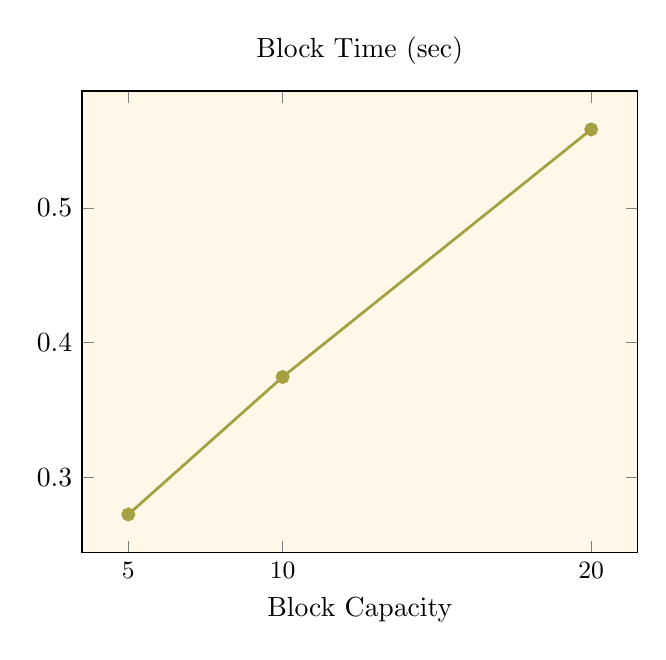
\begin{tikzpicture}
				\begin{axis}[xlabel={Block Capacity},
					title={Block Time (sec)},xtick={5,10,20}, xticklabel style={font=\small} ,width=3.4in,axis background/.style={fill=cosmiclatte}]
					\addplot[mark=*,yellow!60!black, line width=1pt]coordinates{
						(5,27.52293920516968/101)
						(10,19.10346174240112/51)
						(20,13.95952773094177/25)
					};
				\end{axis}
			\end{tikzpicture}
			
		}
		
		\caption{Block Time με block capacities = $\{5, 10, 20\}$, 5 clients και stakes ίσα με 10 για όλους.}
		\label{fig:diagram2}
	\end{figure}
	Πραγματοποιούμε μετρήσεις για το σύστημά μας στις 3 περιπτώσεις που υποδεικνύονται. Χρησιμοποιήσαμε 5 VMs από την cloud υπηρεσία okeanos-knossos.
	\subsection{5 clients - block capacity 5, 10, 20 - ίδια stakes για όλους}
	Στα παρακάτω διαγράμματα των εικόνων \ref{fig:diagram1}, \ref{fig:diagram2} φαίνεται :
	\begin{enumerate}
		\item Το throughput του συστήματος, δηλαδή το πλήθος transactions που ικανοποιούνται στην μονάδα του χρόνου. Υπολογίστηκε ως το πηλίκο του πλήθους των transactions (500) δια του συνολικού χρόνου εκτέλεσης (με έναρξη αμέσως μετά τον τερματισμό του bootstraping).
		\item Το Block Time, δηλαδή τον μέσο χρόνο που μεσολαβεί για την έκδοση νέου block. Υπολογίστηκε ως το πηλίκο του συνολικού χρόνου εκτέλεσης δια του συνολικού πλήθους blocks που δημιουργήθηκαν. 
	\end{enumerate}
Να σημειωθεί ότι ο proxy (για λόγους αντιμετώπισης deadlocks μεταξύ των κόμβων) εισάγει σκόπιμα καθυστέρηση 0.1 second μεταξύ των requests για νέο transaction. Συνεπώς, ο συνολικό χρόνος εκτελεσης περιλαμβάνει και αυτόν τον χρόνο. Με αφαίρεση όλων αυτών των 0.1 seconds, τα διαγράμματα που παράγονται είναι αυτά δεξιά (Without Sleep). Αυτό το 0.1 second δεν είναι απαραίτητο στην περίπτωση που δημιουργούνται σειριακά transactions (και όχι από πολλούς ταυτόχρονα, όπως στο συγκεκριμένο test case). 

\noindent
Από τα διαγράμματα, παρατηρούμε ότι με αύξηση του capacity του block αυξάνεται τόσο το throughput όσο και ο μέσος χρονος δημιουργίας νέου block. Προφανώς, όσο μεγαλύτερο είναι το capacity χρειάζεται περισσότερος χρόνος για να γεμίσει ένα block, ενώ ταυτόχρονα δεν γίνονται και τόσο συχνές δημιουργίες blocks, mining, block broadcasts κλπ. Ως εκ τούτου, περισσότερα transactions μπορούν να εκτελούνται στην μονάδα του χρόνου χωρίς να καθυστερούν εξαιτίας αυτών των διαδικασιών. 
Ενδεικτικά, επειδή χρησιμοποιήθηκαν τέτοιες πληροφορίες για τους υπολογισμούς μας, παρουσιάζεται στην εικόνα \ref{fig:state} το state ενός κόμβου και το συνολικό μέγεθος του blockchain στο τέλος αυτού του πειράματος με capacity 5.
\begin{figure}[h!]
	\centering
	\includegraphics[width=6.5in]{ring.png}
	\caption{State του κόμβου 0 μετά το πείραμα και μέγεθος του blockchain}
	\label{fig:state}
\end{figure}
	\subsection{Κλιμακωσιμότητα του Συστήματος}
	Στη συνέχεια, κάνουμε τα προηγούμενα πειράματα αλλά πλέον με 10 clients. Τα διαγράμματα που παράγονται φαίνονται παρακάτω (εικόνα \ref{fig:diagram5}) και απεικονίζουν για κάθε πλήθος clients το throughput και το blocktime για κάθε διαφορετικό block capacity. Παρατηρούμε ότι εν γένει το thoughput αυξάνεται λίγο με την αύξηση των clients καθώς υπάρχουν περισσότερα transactions προς εκτέλεση στο σύστημα, αλλά η σειριακή τελικά εκτέλεσή τους δεν επιτρέπει κάποια μεγάλη αύξηση στο throughput. Μάλιστα με capacity 5, παρατηρούμε ότι λόγω των πολύ συχνών minings, το σύστημα καταλήγει να έχει μικρότερο throughput. Ως προς το block time, παρατηρούμε ότι αυτό μένει σχεδόν σταθερό για σταθερό capacity, καθώς λόγω της σειριοποίησης των transactions, δεν υπάρχει λόγος να αλλάξει ο χρόνος που χρειάζεται για να γεμίσει ένα block.
		\begin{figure}[t!]
		\centering
		\subfloat[Throughput]{
			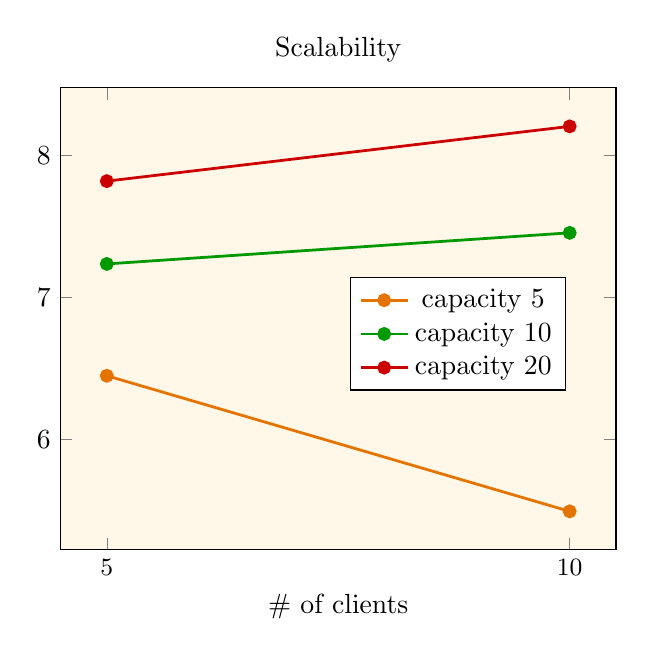
\begin{tikzpicture}
				\begin{axis}[xlabel={\# of clients},
					title={Scalability},xtick={5,10}, xticklabel style={font=\small} ,width=3.4in,axis background/.style={fill=cosmiclatte},    legend style={
						at={(0.91,0.59)}, % move legend to top right corner
						anchor=north east,
					}]
					\addplot[mark=*,orange!90!black, line width=1pt]coordinates{
						(5,500/77.52293920516968)
						(10,1000/181.9258744716644)
			
					};
					\addplot[mark=*,green!60!black, line width=1pt]coordinates{
						(5,500/69.10346174240112)
						(10,1000/134.15281057357788)
						
										};
					\addplot[mark=*,red!80!black, line width=1pt]coordinates{
						(5,500/63.95952773094177)
						(10,1000/121.91563773155212)

					};
					\legend{capacity 5, capacity 10, capacity 20}
				\end{axis}
			\end{tikzpicture}
			
		}
		\subfloat[Block Time]{
			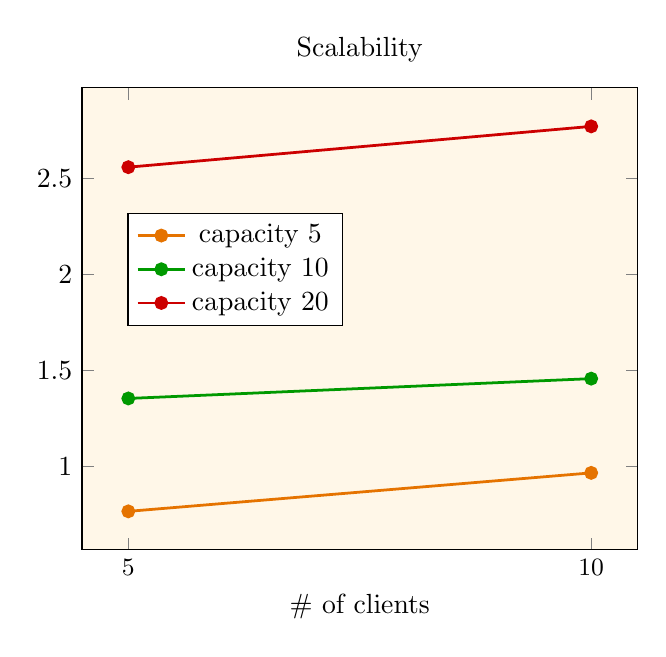
\begin{tikzpicture}
				\begin{axis}[xlabel={\# of clients},
					title={Scalability},xtick={5,10}, xticklabel style={font=\small} ,width=3.4in,axis background/.style={fill=cosmiclatte},    legend style={
						at={(0.47,0.73)}, % move legend to top right corner
						anchor=north east,
					}]
					\addplot[mark=*,orange!90!black, line width=1pt]
					coordinates{
	(5,77.52293920516968/101)
	(10,181.9258744716644/188)

};
\addplot[mark=*,green!60!black, line width=1pt]coordinates{
	(5,69.10346174240112/51)
	(10,134.15281057357788/92)

};
\addplot[mark=*,red!80!black, line width=1pt]coordinates{
	(5,63.95952773094177/25)
	(10,121.91563773155212/44)

};
\legend{capacity 5, capacity 10, capacity 20}
				\end{axis}
			\end{tikzpicture}
			
		}
	
		\caption{Σύγκριση αποτελέσμάτων με χρήση 5 και 10 clients}
		\label{fig:diagram5}
	\end{figure}
	\subsection{Δικαιοσύνη}
	Στη συνέχεια, με χρήση 5 clients και capacity ίσο με 5 (όπως στο πρώτο πείραμα), θέτουμε το stake ενός εκ των participants ίσο με 100 BCC. Στην περίπτωση που όλοι οι nodes είχαν ίδια stakes, μετρούμε πόσες φορές έγινε validator ο καθένας. Το αποτέλεσμα που λαμβάνουμε είναι : [21, 15, 27, 20, 17]. Δηλαδή και οι 5 participants έγιναν περίπου αντιστοιχες φορές validators. Αντιθέτως, αν κάποιος (έστω ο τρίτος κόμβος) έχει stake ίσο με 100, το αποτέλεσμα που λαμβάνουμε είναι : [8, 6, 54, 4, 6], δηλαδή ο τρίτος κόμβος έγινε πολύ περισσότερες φορές validator σχετικά με τους υπόλοιπους. Προφανώς, αυτό είναι άμεσο αποτέλεσμα του consensus αλγορίθμου που χρησιμοποιούμε, δηλαδή το proof of stake, σύμφωνα με το οποίο η πιθανότητα να εκλεγεί κάποιος validator είναι ανάλογη του ποσού stake που δεσμεύει. 
\end{document}